\chapter{Future work and limitations}

\section{Introduction}

In this chapter we present the limitations and possible improvements of FrDataFlow. 
The current implementation is rather limited in its functionality because we wanted to focus on the mapping layer and the possibilities of parallelization using the dataflow engine.
However, multiple improvements can still be made. The signal graphs that can be made in FrDataFlow are still static, e.g. it does not allow the dynamic creation of new signals, the filtering of values or just generally manipulating the timing of value propagation. Every signal always has to emit a value for every set of incoming values. While this already allows for a rich set of programs, these manipulations would be necessary to implement any non trivial program using FrDataFlow. 

\newpage
\section{Dynamically creating signals}

One of the common patterns in reactive programming is the dynamic creation of new signals based on some state or external input. Imagine a button which starts a timer. When this button is pressed, a timer should start running and continuously update the screen with the elapsed time.

This button can be represented as a signal of clicks. Every click is essentially an event, which in terms of reactive programming can be represented as an event being emitted by a signal.

A timer is also a perfect fit for a signal: it is a signal that continuously emits the current elapsed seconds. The tricky part however is that we only want to create this timer when the button is pressed. That means we want to lift the button signal and create a new timer signal only when it is pressed. Maybe another button click stops the timer, or starts a second one, but that is outside the scope of this example.

This pattern of dynamically creating signals is quite common in reactive programming, and unfortunately impossible in FrDataFlow today. A possible improvement would be to enable this, which would mean the signal would have to be added to the topologically sorted signals and be translated to a dataflow node. This would also mean that any existing dataflow nodes upon which this new signal depends would have to be updated to also generate tokens for this new node. Similarly, upon destroying signals, this node and all the references to it would have to be updated. The requirement for a static graph is currently one of the limitations of the dataflow model. There is currently not a single dataflow engine who supports this. It would technically be possible, although it would introduce a considerable amount of bookkeeping overhead. For values that are already being processed by the dataflow engine at the time this reconfiguration happens, it would highly depend on where in the update graph these values currently are to determine if the reconfiguration will be in time to apply for these values. It is therefore impossible to guarantee the correctness of the values already in the update graph at the time of reconfiguration. 

\section{Filtering}

Another common practice is filtering of signals, only letting values through which satisfy a certain predicate. Our current implementation of FrDataFlow models signals as a mapping function which takes a set of inputs and produces a new value for every updated set. Filtering would introduce the possibility of not propagating a value at all if certain criteria are not met. In essence, a signal would no longer provide a lambda that has to return a value, but a lambda that can push values into a type of sink when it wants to. This refactoring would allow for a whole category of powerful constructs, such as taking only the first n values, throttling signals, etc. 

An example visualization of the filter function in RxJs can be seen in figure  \ref{fig:futurework-filtering-filter}. 

\begin{figure}[h!]
	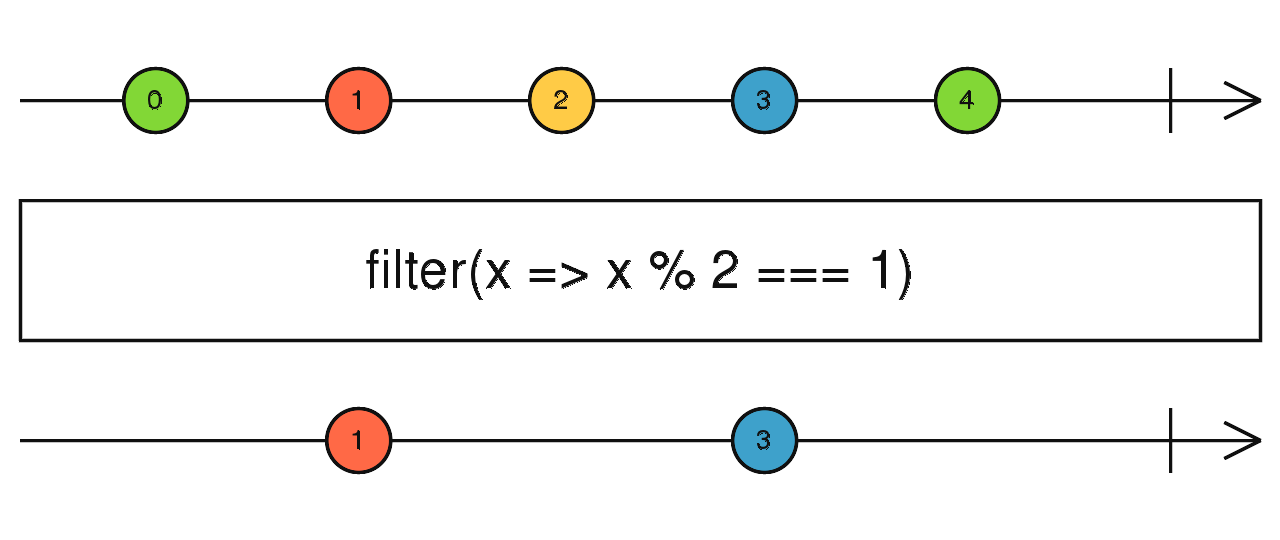
\includegraphics[width=\textwidth]{images/FutureWork-Filtering-Filter.png}
	\caption{A timeline diagram of the \textit{filter} operator in RxJs}
	\label{fig:futurework-filtering-filter}
\end{figure}

We see at the top a signal which produces a stream of numbers. If we create a new signal that filters these numbers using the filter function, we get a new stream of numbers that only contains those that satisfied the predicate. When the number 0 is pushed into the signal lambda, it does not propagate it into the sink of the child signal, which means the value does not go through. 

To implement this pattern in our mapping layer, we would have to ensure that dataflow nodes don't always have to produce new tokens when they are invoked, and a way for nodes to indicate when this should happen or not. However, there is no technical reason why the dataflow engine should not be able to handle this: it is simply the presence of tokens that determines which nodes are invoked, so not emitting these tokens would essentially implement the filtering behavior we have described. Unfortunately, the current design of FrDataFlow does not allow the production of zero or more than 1 output token for 1 input token, because of the design of the lift operator. This operator would have to be redesigned to use a sort of sink model where values can be pushed into, allowing each lift operator to decide the amount of output values it produces per incoming value. The value of each signal would then no longer be determined by the return value of the lift operator, but rather by the values that get pushed into the sink object that is provided to the lift function. This approach has not been validated yet, but we propose that the model does support it.


\section{Conclusion}

In this chapter we have shown how FrDataFlow is still a basic language that does not support some powerful concepts such as the dynamic creation of signals or the filtering of values.
If these concepts were to be introduced, they would allow for an implementation of most of the techniques commonly found in other reactive libraries or languages.

This initial version of FrDataFlow has focused mostly on the practical mapping layer from reactive programming to the dataflow model. The dynamic creation of signals is possible in theory, but would have to make trade-offs regarding the correctness of values already being processed by the dataflow engine. Secondly, filtering could be implemented using a sink model in FrDataFlow, with the necessary updates to the mapping layer so it would generate tokens based on the values that get pushed into the sink. However, both of these proposed solutions have not been explored and are therefore not validated.  